\documentclass{article}
\usepackage[backend=bibtex]{biblatex}
\usepackage{amssymb}
\usepackage{listings}
\usepackage{graphicx}
\author{Fredrik Kortetjarvi \& Rohullah Khorami}
\title{Exercise 1}
\addbibresource{Exercise.bib}
\begin{document}
    \maketitle
    \section{}
        Citoday breach this contains 226,883,414 accounts. The breach used socail engineering to get the information they used mailinator to 
        mail fake mails to users in a guitar forum there it could send out. This kind of breaches cant be stoped becasue this is using tricks 
        to trick the brain of people so they give out the information for free. this can only be improved but not fixed.\cite{cit0day} 
    \section{}
        The program generate a picture with a name IOCCC in raytracing.
        We used cmake to make this into a ppm file then 
        display it in gimp to see the picture that was created see figure \ref{fig:Zucker}. We found the makefile
        on the internet which was a programming contest. The program use functions to make a program to 
        draw graphics into a ppm file that is a picture.\cite{zucker}
        \begin{figure}
            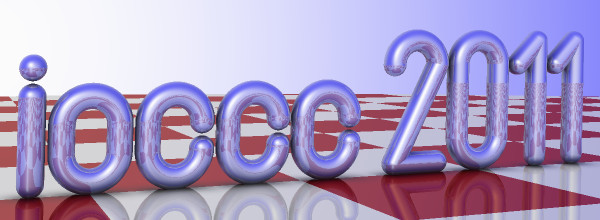
\includegraphics[width=\linewidth]{image.jpg}
            \caption{Raytracing.}
            \label{fig:Zucker}
        \end{figure}
    \section{}
        The Key that Eve guessed indeed decrypts the cipher text to "LATER".
        we checked the result in java program and on pen and paper. The program explaind in Task 4.\newline
        \begin{math}
        11=(x-84)mod26\Leftrightarrow T=11\rightarrow L , newkey=19 \rightarrow T\newline
        0=(x-82)mod26\Leftrightarrow T=25\rightarrow Z , newkey=16 \rightarrow Q\newline
        19=(x-84)mod26\Leftrightarrow T=21\rightarrow V , newkey=20 \rightarrow U\newline
        4=(x-83)mod26\Leftrightarrow T=3\rightarrow D , newkey=17 \rightarrow R\newline
        17=(x-72)mod26\Leftrightarrow T=18\rightarrow S , newkey=8 \rightarrow I\newline
        \end{math}\newline

        First attempt\newline
        Plain Text = LZVDS - 11 25 21 3 18\newline
        Key = TRTSH - 84 82 84 83 72\newline
        Cipher Text = EQNVZ - 4 16 13 21 25\newline

        Take out the key\newline
        Plain text = LATER - 11 0 19 4 17\newline
        Key = TQURI - 19 16 20 17 8\newline
        Cipher Text = EQNVZ - 4 16 13 21 25\newline

        \begin{math}
            T=(x-k)mod26+65\newline
            78-65=13=(x-84)mod26+65\Leftrightarrow T=78\rightarrow N , x=71 \rightarrow G\newline
            69-65=4=(x-82)mod26+65\Leftrightarrow T=69\rightarrow E , x=86 \rightarrow V\newline
            86-65=21=(x-84)mod26+65\Leftrightarrow T=86\rightarrow V , x=79 \rightarrow O\newline
            69-65=4=(x-83)mod26+65\Leftrightarrow T=69\rightarrow E , x=87 \rightarrow W\newline
            82-65=17=(x-72)mod26+65\Leftrightarrow T=82\rightarrow R , x=89 \rightarrow Y\newline
            \end{math}\newline
        Plain text = NEVER - 78 69 86 69 82\newline
        Key = TRTSH - 84 82 84 83 72\newline
        Cipher text = GVOWY - 71 86 79 87 89\newline
    \section{}
    \lstinputlisting[language=Java,breaklines=true]{OtpInputStream.java}
    \section{}
    All steps to find public key and private key\newline
        
    \textbf{1.}\newline
        \begin{math}
         p = 7 , q = 11 
        \end{math}\newline
        
        \textbf{2.}\newline
        \begin{math}
         N = P*q = 77 
        \end{math} \newline
        
        \textbf{3.}\newline
        \begin{math}
         W = (p-1)(q-1) = 60
        \end{math}\newline
        
        \textbf{4.}\newline
        To decide an E value thoug we should know that E must be a prime number and GCD(E,W) = 1  and 1 $<$ E $<$W
        we asume that E = 53 and GCD(53,60) = 1\newline
        
        \textbf{5.}\newline
         D = 1/E mod W =$>$ ED = 1 Mod W  =$>$ D = ((W*i)+1)/E\newline
        We check i value step by step or we count the number of prime numbers from 1 to 53. The i Value must be an Integer.
        In this situation there are 15 prime number before 53 than the i value become 15.\newline
        i = 15 and D = ((60*15)+1)/53 = 17.  D = 17\newline
        
        \textbf{6.}\newline
        public key = {E,N} = {53,77}\newline   
        private key = {D,N} = {17,77}\newline
        
        \textbf{7.}\newline
        Exemple we want to encrypt a message "M" there M$<$N and  M = 10.\newline
        
        Encryption:\newline
        \begin{math}
            C = T ^ E mod N \newline 
        \end{math}
            C = cipher text\newline
            T= Message = 10\newline
            E = Exponent = 53\newline
            N= p*q = 77\newline
        \begin{math}
            C = 10^{53}mod77  = 54\newline 
        \end{math}
            cipher text = 54\newline
        
            Decryption:\newline
        \begin{math}
            T = C ^ D mod N \newline 
            T = 54^{17} mod 77 = 10
        \end{math}\newline
        T = message = 10. 
    \section{}
    Euclidean algorithm is an efficient method for computing the Greatest Common Divisor (GCD) of two integer. The largest number that divides them both without a remainder.\newline
    Euclidean alogorithm is used in RSA cipher to find an exponent E so that the E Should not be a factor of $\phi(n)$, in other word $GCD(E,\phi(n)) = 1$ 
    which means that we use Euclidean algorithm to find a prime E that the GCD between Exponent and $\phi(n)$ (in our case it is W in task 5) should be equal to one.
    \section{}
    \section{}
    Nothing
    \section{}
    The page the we found is www.afg.se which is an engineering page and we search this page on google we
    get exclamation mark in the address field. We checked the certificate chain and the issue with this page is that it has certificate chain but the certificate is not verified and the other issue with the page is that the images in the page is not safe. from "afg.se" to "R3" to "DST root CA X3". 
    The public key in afg.se is RSA (2048 bits) which is not secure becuase it is breakable hexa codes.\cite{AFG}
    \begin{figure}
        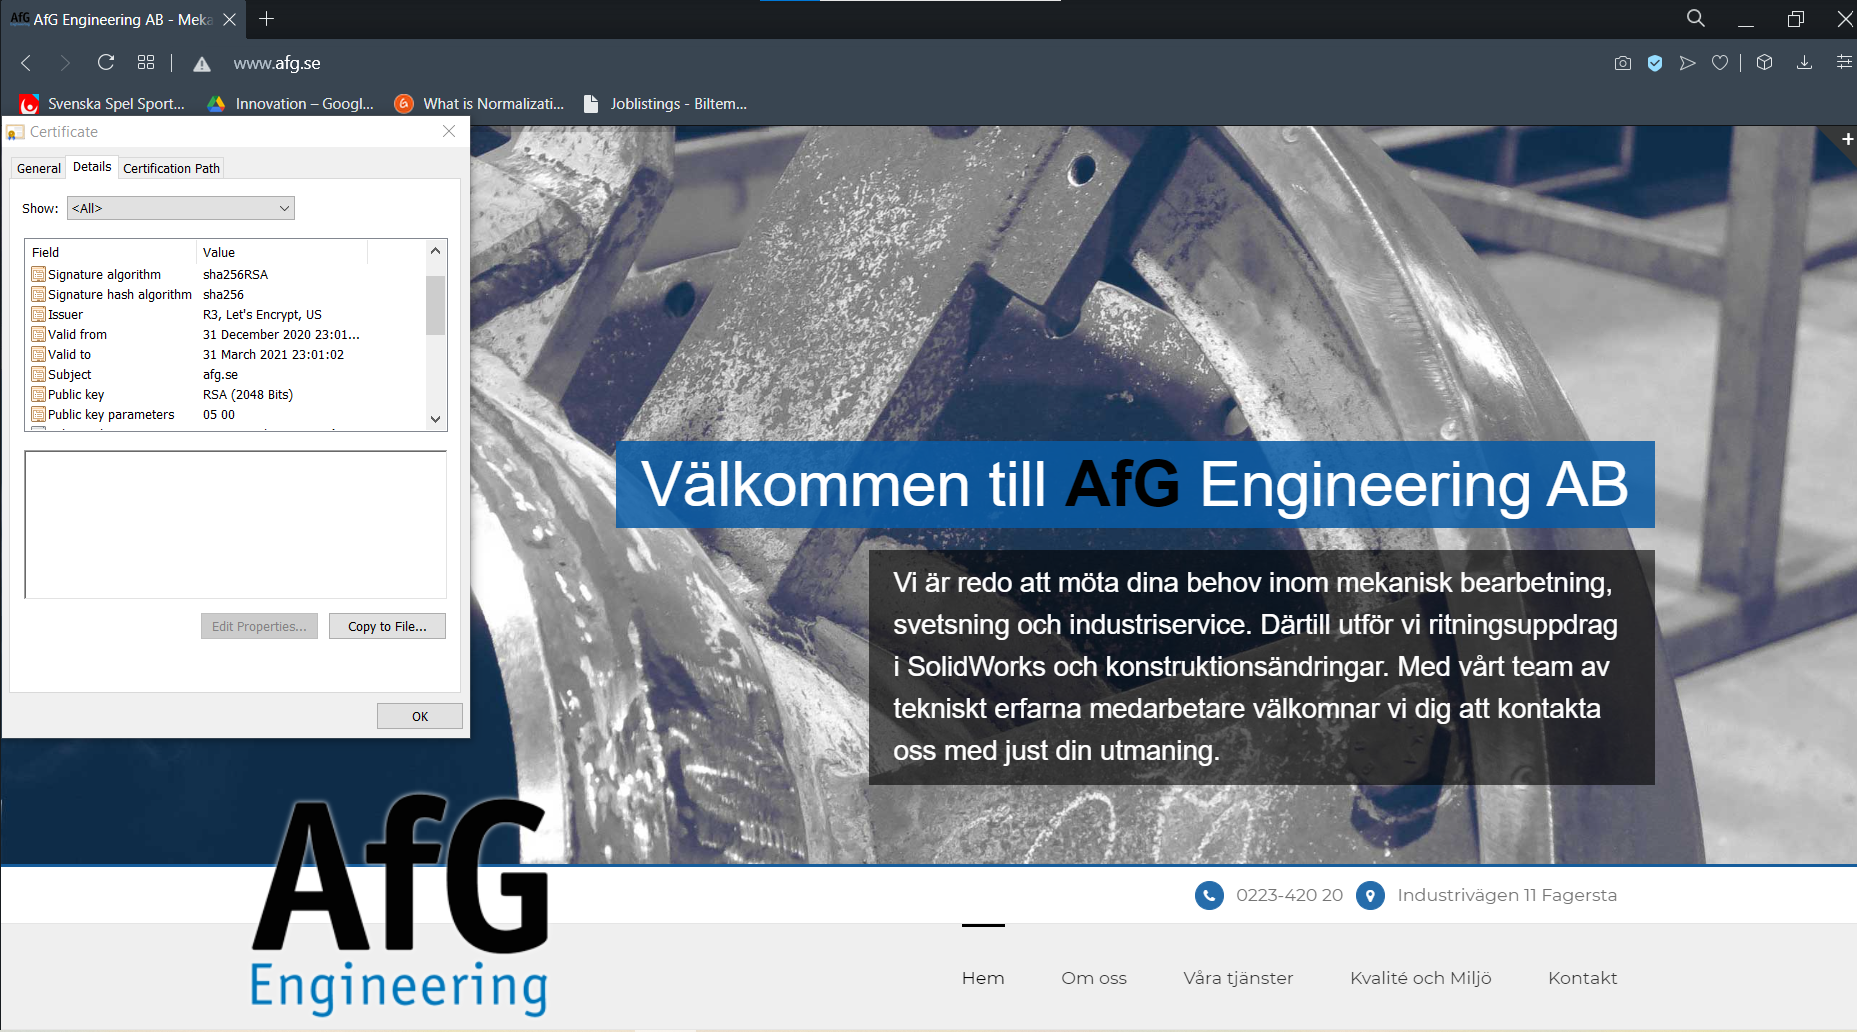
\includegraphics[width=\linewidth]{afg.png}
        \caption{AfG.se}
        \label{fig:AfG}
    \end{figure}
        \newpage
        \printbibliography
\end{document}